\documentclass[../../main.tex]{subfiles}

\begin{document}
\section{Moto Circolare}
\[
    s(t) = \theta(t)R , \begin{cases}
        x(t) = R\cos(\theta(t)) \\
        y(t) = R\sin(\theta(t))
    \end{cases}
\]
Velocità angolare media = $\omega_m = \dfrac{\theta(t_f) - \theta(t_i)}{t_f - t_i}$ \\
$\omega = \dfrac{d\theta}{dt} \implies $ se uniforme $\omega$ è \textbf{costante}. \\
\[
    \bar v = v_s\cdot\bar u_t = \dfrac{ds}{dt}\bar u_t = R\dfrac{d\theta}{dt}\cdot\bar{u}_t
\]
\[
    \textcolor{red}{v_s = R\omega}
\]
$
    a_t = 0, \ \ a_n = \dfrac{v^2_s}{R} = \dfrac{\omega^2R^2}{R} = \omega^2R
$ uniforme \\
$
    a_t = \dfrac{dv_s}{dt} = \dfrac{Rd\omega}{dt} \ \ \ a_n = \dfrac{v_s^2}{R} = \omega^2R
$
\[
    \alpha \textit{ accelerazione angolare } = \dfrac{d\omega}{dt} \implies \ a_t = R\alpha \ \ \ a_n = \omega^2R
\]
\[
    \omega = \omega_0 + \int_{t_0}^{t} \alpha dt = \omega_0 + \alpha(t - t_0)
\]
\subsection{Notazione vettoriale nel moto circolare}
\begin{figure}[h!]
    \centering
    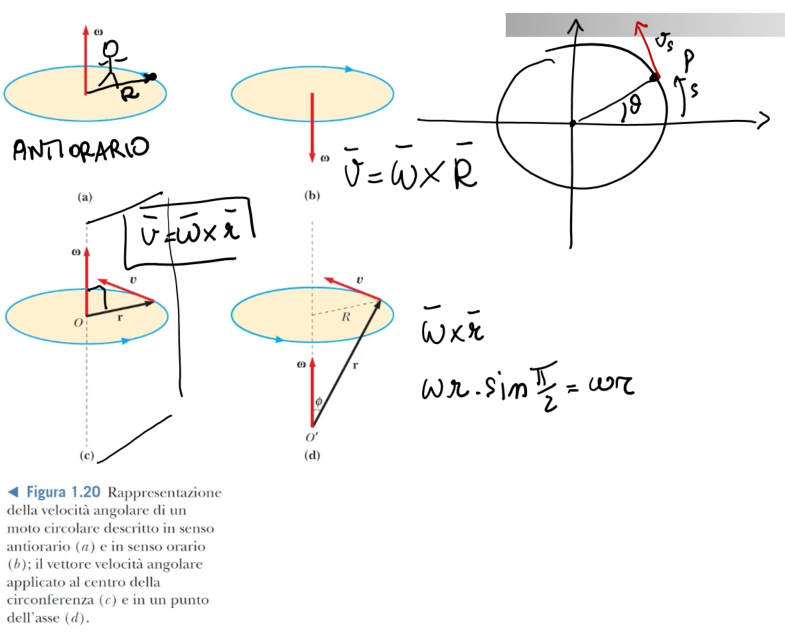
\includegraphics[width=0.5\textwidth]{moto_circolare2.png}
\end{figure}
\[
    v_s = \omega R
\]
\[
    \bar{v} = v_s \cdot \bar{u}_t
\]
\[
    \bar a = \dfrac{d\bar v}{dt} = \dfrac{\bar\omega\times\bar r}{dt} = \dfrac{d\bar \omega}{dt}\times\bar r + \bar\omega\times\dfrac{d\bar r}{dt}
\]
$wr\cdot\sin\frac{\pi}{2} = wr \ \ \ \bar\alpha = \dfrac{d\bar\omega}{dt} \ \ \ \bar a = \bar\alpha\times\bar r + \bar\omega\times\bar v \implies \bar a = \alpha\cdot r + \bar\omega\times\bar v$
\[
    \bar a_t = \bar\alpha\times\bar r
\]
\[
    \bar a_n = \bar{\omega}\times\bar v \ \ \ \textit{accelerazione centripeta}
\]
\end{document}